\section{Khám phá dữ liệu và kiểm tra ảnh trùng}
Phần khám phá dùng mirror \code{uoft-cs/cifar100} tại revision cố định. Hash toàn bộ pixel và nhãn theo thứ tự của cả 50.000 ảnh development và 10.000 ảnh test khớp với dữ liệu Toronto trong metadata của các lượt chạy. Tất cả ảnh đều là RGB $32\times32$. Mỗi lớp có 450 ảnh train, 50 ảnh validation và 100 ảnh test, nên không có mất cân bằng theo số lượng fine classes. Tuy nhiên, cân bằng số mẫu không bảo đảm các lớp có độ khó tương đương.

\begin{figure}[htbp]\centering
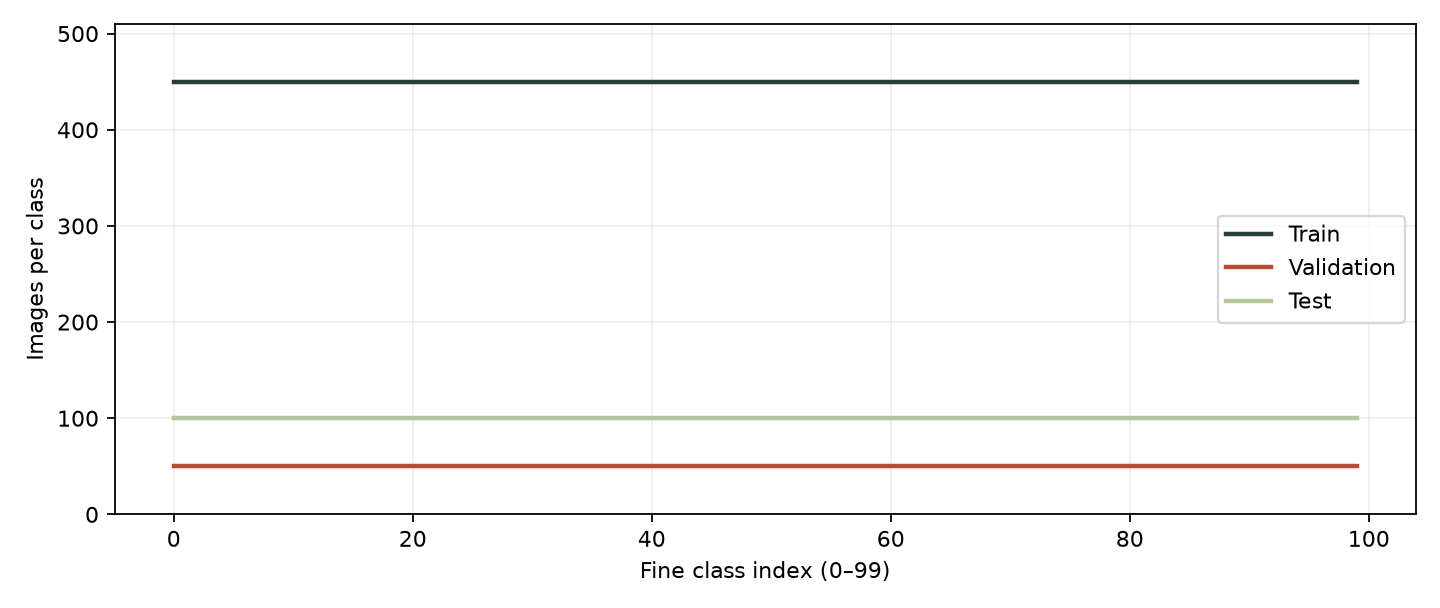
\includegraphics[width=.92\textwidth]{analysis/class_counts.png}
\caption{Số ảnh từng fine class sau split. Các lớp có cùng số ảnh trong mỗi split.}
\end{figure}
\begin{figure}[htbp]\centering
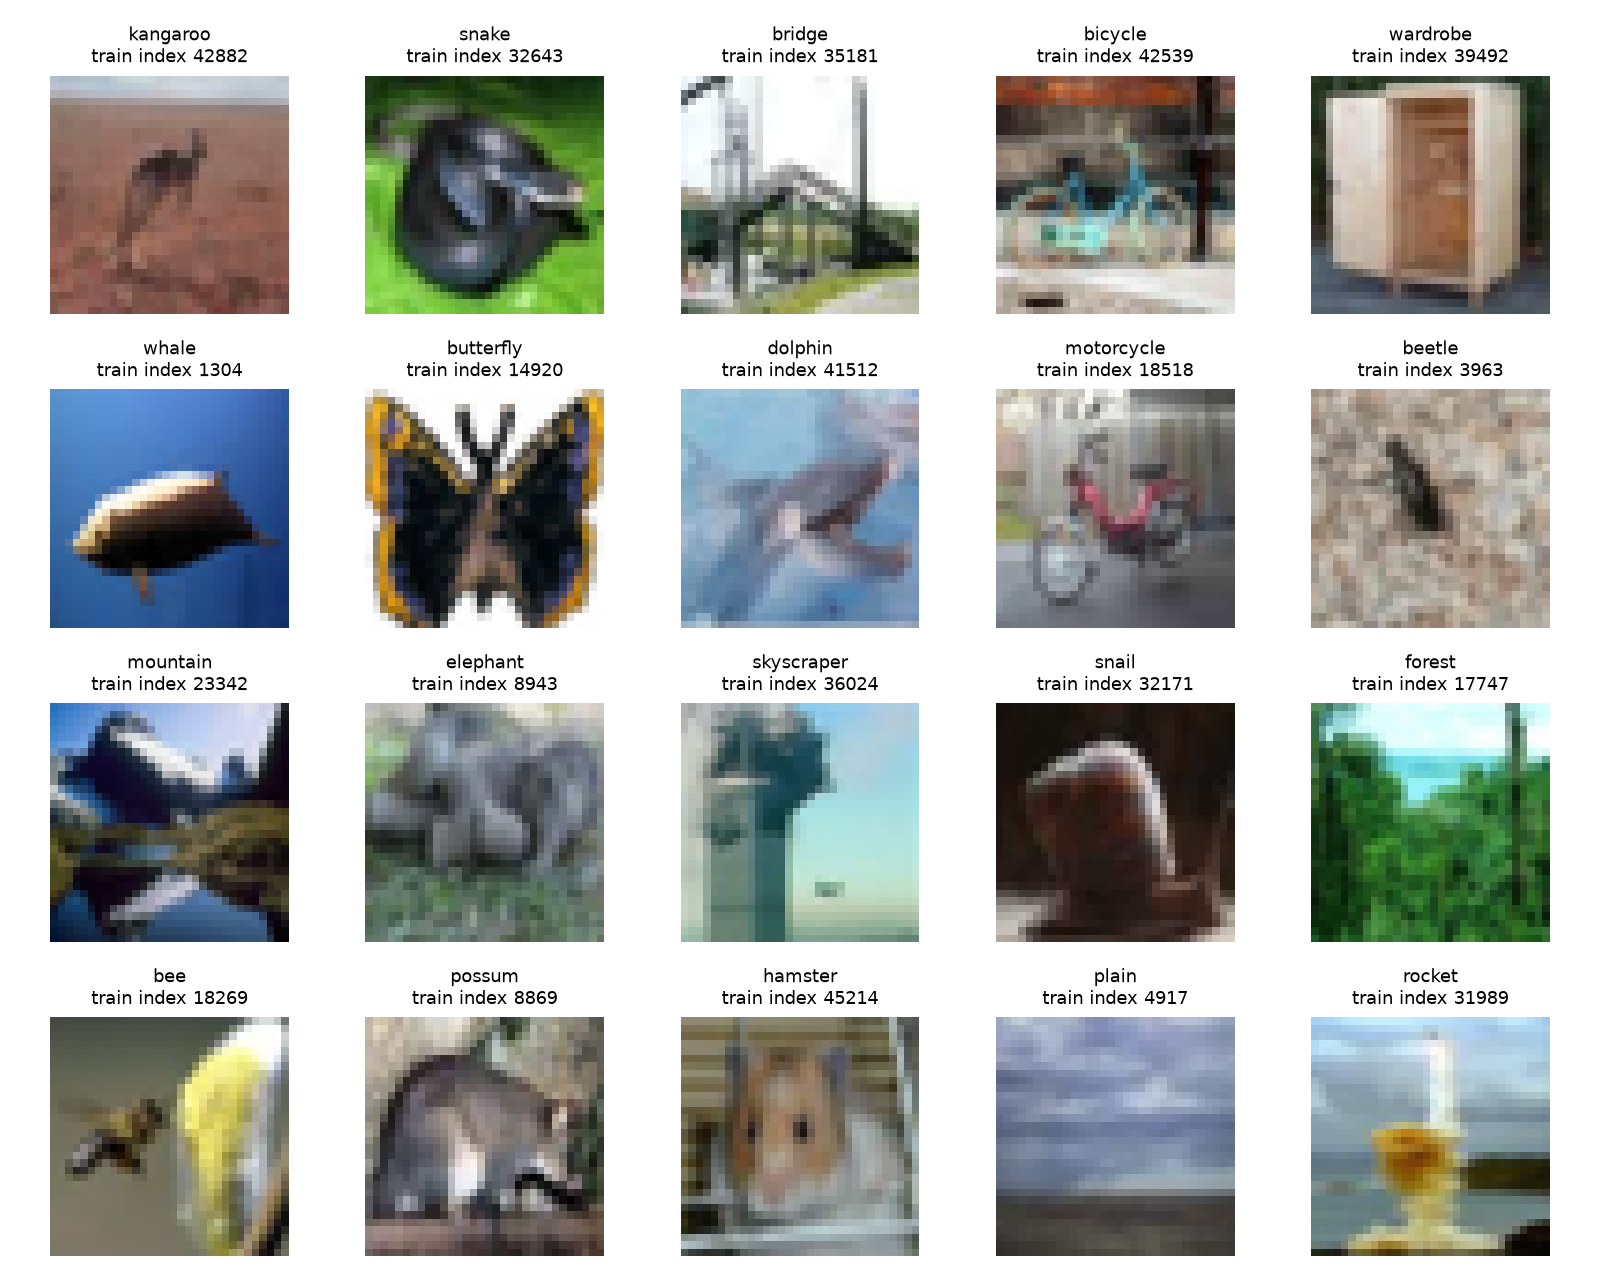
\includegraphics[width=.78\textwidth]{analysis/training_samples.png}
\caption{Hai mươi ảnh train chọn bằng seed 2026, kèm nhãn và chỉ số gốc. Ảnh được phóng lớn để quan sát; chi tiết phân biệt một số lớp vẫn hạn chế.}
\end{figure}

Kiểm tra SHA256 trên RGB bytes phát hiện 14 ảnh lặp nội dung trong tập development 50.000 ảnh. Trong split đã đo có 2 nội dung ảnh trùng giữa train và validation, 10 nội dung trùng giữa train và test, không có trùng validation--test. Test có 9.998 nội dung ảnh duy nhất trên 10.000 bản ghi. Đây là kiểm tra trùng pixel hoàn toàn, chưa đánh giá near duplicates. Vì vậy, các split tách rời về chỉ số nhưng không hoàn toàn tách rời về nội dung ảnh.

Bộ split và checkpoint đã công bố được giữ nguyên. Kiểm tra độ nhạy bổ sung loại 10 ảnh test trùng train, giữ 9990 prediction của cùng các checkpoint. ResNet18 full đạt 79.009\%, so với 78.970\% ban đầu; Swin-T full đạt 86.677\%, so với 86.630\% ban đầu. Chênh lệch nhỏ trong kiểm tra này không chứng minh quy trình hoàn toàn không có leakage: hai nội dung trùng train--validation vẫn có thể ảnh hưởng chọn checkpoint. Không gọi đây là kết quả train lại sau loại trùng.

Một protocol tiếp theo cần nhóm các ảnh trùng trước khi chia dữ liệu và đo lại toàn bộ đối chứng. Không thay split sau khi xem test rồi gộp phép đo mới với bảng cũ. Các chỉ số và danh sách ảnh trùng nằm trong \code{analysis/dataset.json}, \code{overlap.json} và \code{sensitivity.json}.
